\chapter{Návrh a implementace}\label{chapter:navrh}
V~této kapitole budou popsány změny návrhu programu, které se skládají z~navržených změn podle požadavků frontendového týmu a návrhu chybějících funkcí. Dále bude popsána implementace změn návrhu a chybějících funkcí. Nakonec bude popsán návrh a následná implementace funkcí, které jsou zaměřené na zlepšení kvality výsledného softwaru.

Při úpravách současného návrhu byl proveden  velký počet změn různé významnosti. V~této kapitole budou uvedeny klíčové změny. Při implementaci návrhu autorovi pomohlo přečtení doporučené literatury.\cite{pro-spring-boot-2}

\section{Úpravy podle požadavků frontendového týmu}\label{navrh:upravy}
    V~této sekci budou popsány navržené změny podle požadavků frontendového týmu a jejich následná implementace.
    
    \subsection{Interval}\label{navrh:upravy:interval}
        \begin{figure}\centering
	        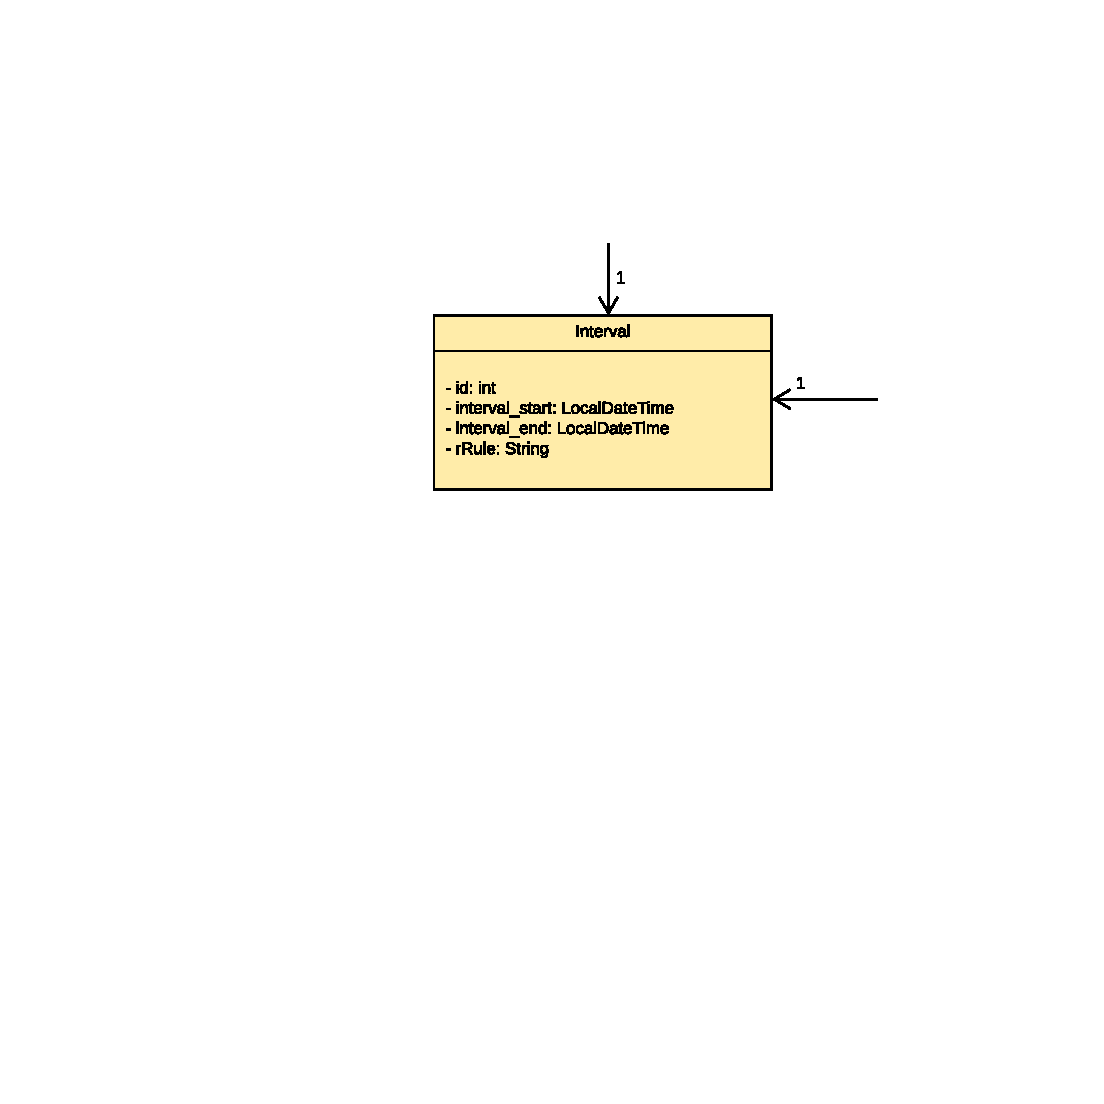
\includegraphics[width=0.7\textwidth]{pdfs/Interval2}
	        \caption[Nový návrh entity \texttt{Interval}]{Nový návrh entity \texttt{Interval}}\label{image:Interval2}
        \end{figure}
        \begin{figure}\centering
	        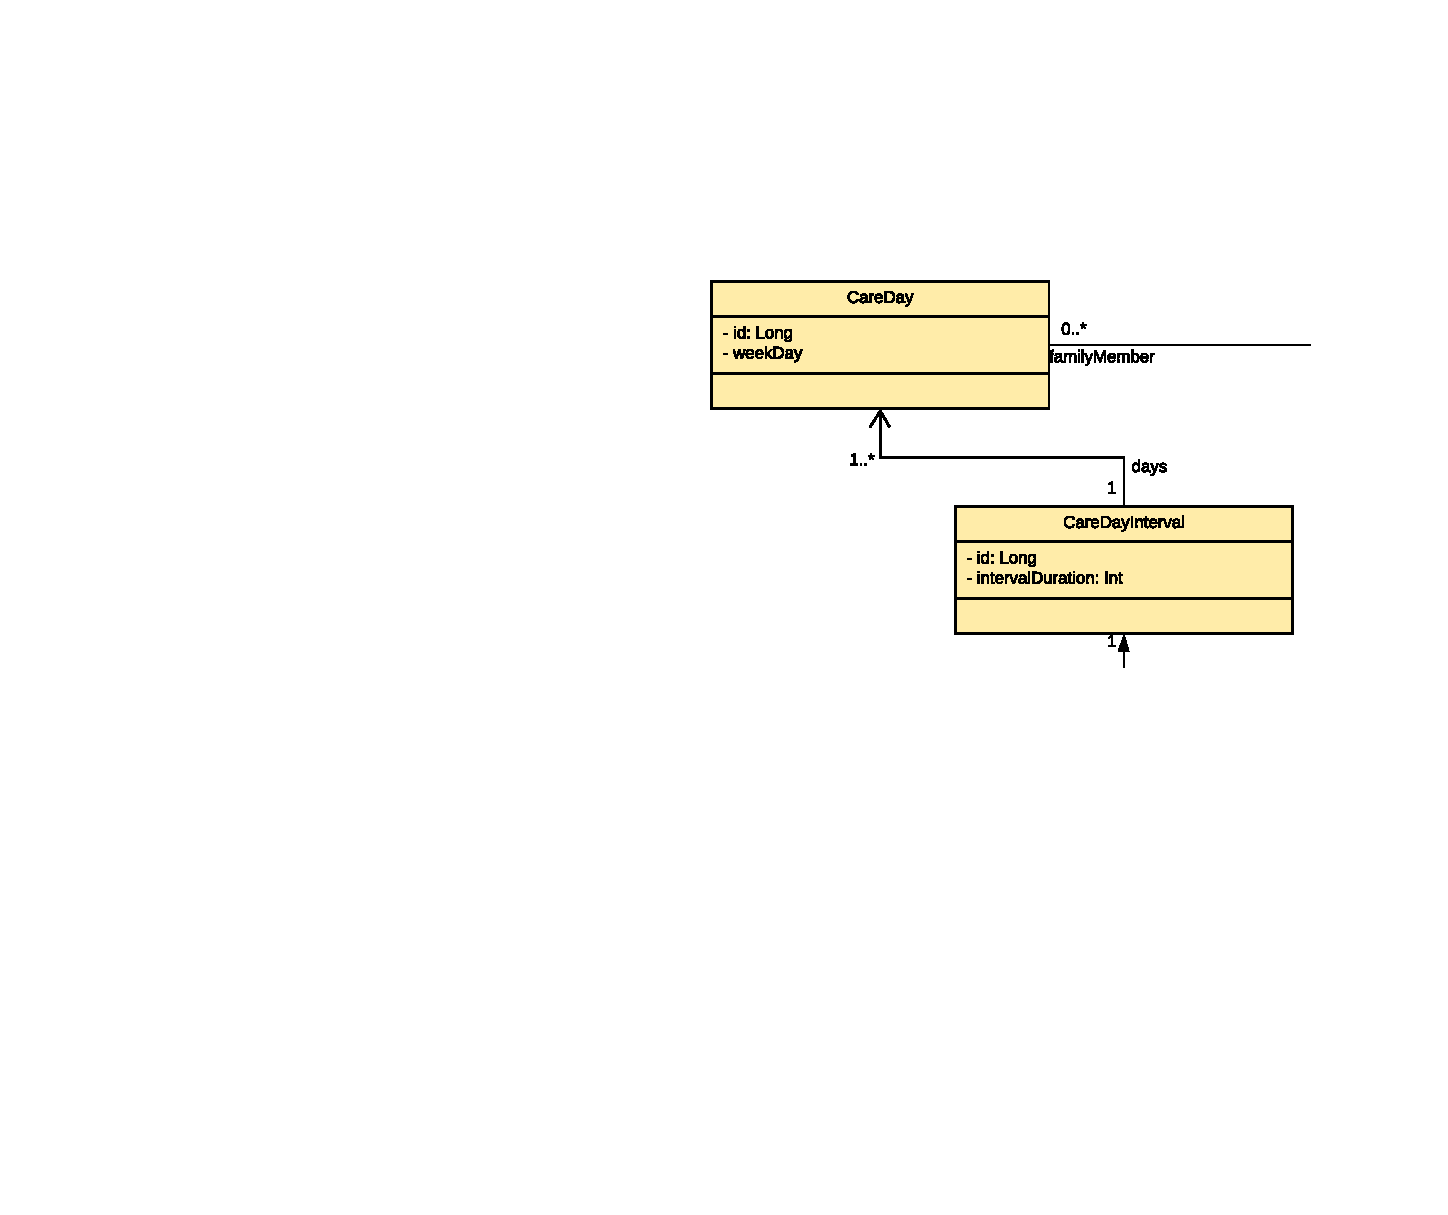
\includegraphics[width=0.8\textwidth]{pdfs/CareDayInterval}
	        \caption[Návrh entity \texttt{CareDayInterval}]{Návrh entity \texttt{CareDayInterval}}\label{image:careDayInterval}
        \end{figure}
        První změnou je nový návrh entity \verb|Interval|. Původní návrh nevyhovoval svou složitostí a zároveň jenom částečným pokrytím možných případů užití (viz~obrázek~\ref{image:Interval1}). Podrobně tento problém byl popsán v sekci \ref{analyza:pozadavky:interval}. Entita řešila několik samostatných problémů najednou: pravidla pečovatelských dnů rodičů a klasické intervaly definující pravidla opakování nebo jednorázovou událost. Proto entita \verb|Interval| byla rozdělena do~dvou samostatných částí.
        První část se zabývá pravidly pro pečovatelské dny rodičů (viz obrázek \ref{image:Interval2}). Tento typ intervalu bude podrobně popsán v~sekci \ref{navrh:upravy:caredays}. Ostatní případy použití intervalů nevyžadují, ani specifické atributy, ani specifický rozsah možných pravidel, proto ostatní případy použití řeší stejná entita -- \verb|Interval| -- (viz obrázek \ref{image:Interval2}).
    
        Nový návrh entity \verb|Interval| je kompilovaný, proto je potřeba podrobně popsat použitou architekturu. Nový návrh je postaven na jiném principu, kde časové rozmezí může být reprezentováno dvěma způsoby. Oba dva způsoby vyžadují uvedení začátku intervalu. Tento parametr je povinný. První způsob vyžaduje kromě začátku intervalu i konec intervalu. Takovým způsobem můžeme definovat jednorázový interval po sobě jdoucích dnů. Druhý způsob vyžaduje zadání pravidla opakování. Takto můžeme definovat stejný interval, ale mnohem složitějším způsobem. Na druhou stranu, pomocí takového pravidla můžeme definovat libovolně složitý interval. 
        Například zmíněný v~sekci \ref{analyza:pozadavky:interval} interval, který se bude opakovat každý poslední den měsíce. Výsledný návrh sestavení intervalu vyžaduje, aby byl zadán buď jenom konec intervalu, nebo aby bylo zadáno jenom pravidlo opakování. V~případě, že tyto dva parametry budou zadány najednou, server vyhodí chybu a zastaví vytvoření nesprávného intervalu. Pravidlo opakování je reprezentováno pomocí textového řetězce, který má být zadán podle standardu {RFC 5545}.\cite{recurrence-rule} Pro pohodlné sestavení pravidel opakování při testování aplikace byl navržen a implementován {interní DSL jazyk}\footnote{DSL jazyk využívající obecný programovací jazyk.}. Tento jazyk bude podrobně popsán v sekci \ref{navrh:zmeny:dsl}.
        \begin{figure}[h]
                \begin{minted}[frame=lines,
        framesep=2mm,
        baselinestretch=1.2,
        fontsize=\footnotesize,
        linenos]{java}
@Scheduled(cron = "\${scheduled.alimonyFactory.cronExpression}")
fun createAlimonyForEachAlimonySetting() {
    logger.info("Started scheduled alimony creation process;")
    val alimony = alimonySettingRepository
                        .findAllByEnabledTrue()
                        .map { it.createAlimony() }
    if (alimony.isNotEmpty()) {
        alimonyRepository.saveAll(alimony)
    } else {
        logger.debug(
            "AlimonyFactory didn't find any AlimonySetting to work with;"
            )
    }
}
                \end{minted}
                \caption{Ukázka metody vytvářející instance alimentů} 
                \label{code:create-alimony}
            \end{figure}
        
    \subsection{Alimenty}\label{navrh:upravy:alimenty}
        Druhou důležitou úpravou současného návrhu je změna entity \verb|Alimony|. Tyto úpravy se dotykají entity samotné a spravování instancí této entity.
    
        \subsubsection{Úprava entity}
            Za účelem zvýšení samostatnosti instancí entity \verb|Alimony| byla přidána závislost na entitu \verb|Family|. Také byl přidán atribut \verb|value|, který kopíruje z~entity \verb|AlimonySetting| částku, která má být uhrazena jedním z rodičů. Příčinou přidání tohoto atributu je existence možnosti aktualizace nastavení alimentů, což působí zneplatnění již existujících instancí alimentů. V~případě, že rodiče změní hodnotu v~nastavení alimentů, ztratí se~možnost zjistit hodnoty alimentů, které byly vytvořeny do změny.
            
        \subsubsection{Spravování alimentů} 
            V~této sekci bude popsán návrh třídy, která se věnuje pravidelnému vytváření alimentů.
            
            Všechny instance alimentů je potřeba vytvářet pravidelně. Proto vytváření bylo objednáno do jednoho procesu, který je stejný pro všechny instance. Proces vytváření alimentů zajišťuje specifická metoda, která se nachází ve~třídě \verb|AlimonyFactory| (viz obrázek \ref{code:create-alimony}). Metoda vyhledává všechny aktivní instance \verb|AlimonySetting| a pro každou vytvoří instanci entity \verb|Alimony|. 
            
            \begin{figure}
                \begin{minted}[frame=lines,
        framesep=2mm,
        baselinestretch=1.2,
        fontsize=\footnotesize,
        linenos]{yaml}
\# Cron expression: at 01:01 AM on the 1st day of every month
scheduled.alimonyFactory.cronExpression=0 1 1 1 * ?
                \end{minted}
                \caption{Ukázka konfigurace \texttt{cron} výrazu pro plánování vytváření alimentů} 
                \label{code:cron-expression}
            \end{figure}
            Vytvářeni alimentů má být pravidelné a nemusí vyžadovat účast člověka. Proto byla využita funkcionalita frameworku Spring, která poskytuje možnost plánování automatického spouštění.\cite{spring-scheduling} Anotace \verb|@Scheduled| vytváří z~dané metody komponentu, která se vykonává podle uvedeného pravidla. Existuje několik podporovaných typů pravidel. 
            Například nastavení intervalu mezi nastartováními nebo mezi ukončeními. Ale pro plánovaní vytváření alimentů je potřeba nastavit konkrétní den měsíce nebo roku, který se bude opakovat. Proto bylo zvoleno \verb|cron| pravidlo, které je také touto podporováno anotací.\cite{cron-expression} Tento výraz je textovou řádkou, která se skládá z~čísel oddělených mezerami reprezentujících čas spouštění.
            Toto pravidlo nebylo zadáno přímo do kódu. Pro přidání možnosti pohodlné konfigurace pravidla byla definována proměnná prostředí, která se nachází v~konfiguračním souboru příslušného profilu (viz obrázek \ref{code:cron-expression}). Implementace byla provedena podle návodu z~knihy~\cite{sbr:spring-task-scheduling}. Podrobněji budou profily popsány v~sekci \ref{navrh:profily}.
         
            \begin{figure}
                \begin{minted}[frame=lines,
        framesep=2mm,
        baselinestretch=1.2,
        fontsize=\footnotesize,
        linenos]{yaml}
scheduled.alimonyFactory=true
                \end{minted}
                \caption{Ukázka proměnné prostředí zapínající \texttt{AlimonyFactory}} 
                \label{code:alimony-factory-true}
            \end{figure}
            Byla přidána možnost měnit čas spouštění metody pomocí konfiguračního souboru, ale také bychom potřebovali mít možnost vypnout tuto metodu, například pro robustní testování. Proto byla přidána třída, která vytváří instanci tříd obsahující automaticky spustitelné metody. Třída je definována jako komponenta frameworku Spring a každá její metoda je určena pro vytváření instancí jiných tříd podle předem definované podmínky.
            V~případě, že podmínka má hodnotu \verb|false|, příslušná třída se nevytváří.
            Pro vytváření třídy \verb|AlimonyFactory| byla definována podmínka, která ověřuje, jestli proměnná \verb|scheduled.alimonyFactory| je nastavená na hodnotu \verb|true| (viz obrázek \ref{code:alimony-factory-true}). V~případě, že tato proměnná nebyla definována pro aktuální profil aplikace, proměnná se automaticky nastaví na hodnotu \verb|false| a instance třídy \verb|AlimonyFactory| nebude vytvořena.
        
    \subsection{Pečovatelské dny}\label{navrh:upravy:caredays} % PECOVATELSKE DNY
        V~předchozím návrhu implementace dlouhodobých nastavení pečovatelských dnů pro rodiče a jednorázových změn byly reprezentované pomocí stejné entity (viz obrázek \ref{image:caredays1}). Problém je právě ve sjednocení několika problémů do~jednoho. Proto bylo rozhodnuto rozdělit řešení do dvou částí. Výsledný návrh se~skládá ze čtyř entit (viz obrázek \ref{image:caredays2}):
        \begin{itemize}
            \item \texttt{CareDaysSetting}, reprezentující dlouhodobé nastavení pečovatelských dnů;
            \item \texttt{CareDayInterval}, reprezentující interval pečovatelských dnů pro dlouhodobé nastavení;
            \item \texttt{CareDay}, reprezentující jeden pečovatelský den pro dlouhodobé nastavení;
            \item \texttt{CareDayChange}, reprezentující změnu pečovatelských dnů.
        \end{itemize}
        Dlouhodobá nastavení pečovatelský dnů rodičů již byla zmíněna v~sekci \ref{navrh:upravy:interval}. Nastavení se skládají z~po sobě jdoucích dnů, kde každý den má odkaz na~jednoho rodiče, který má v~péče dítě v~tento den. Interval je uchováván v~entitě \verb|CareDaysSetting|, která reprezentuje nastavení pečovatelských dnů rodičů pro konkrétní rodinu. Tato nastavení definují implicitní nastavení pečovatelských dnů, podle kterých se vyplní kalendář rodiny.
        
        Změny pečovatelských dnů jsou reprezentovány entitou \verb|CareDayChange|. Interval změny nebo pravidlo opakování změny je reprezentován pomocí entity \verb|Interval|. Každá změna se~vztahuje ke konkrétnímu členovi rodiny a instanci nastavení pečovatelských dnů příslušné rodiny.
        
    \subsection{Oznámení}\label{navrh:upravy:notification}
        \begin{figure}\centering
	       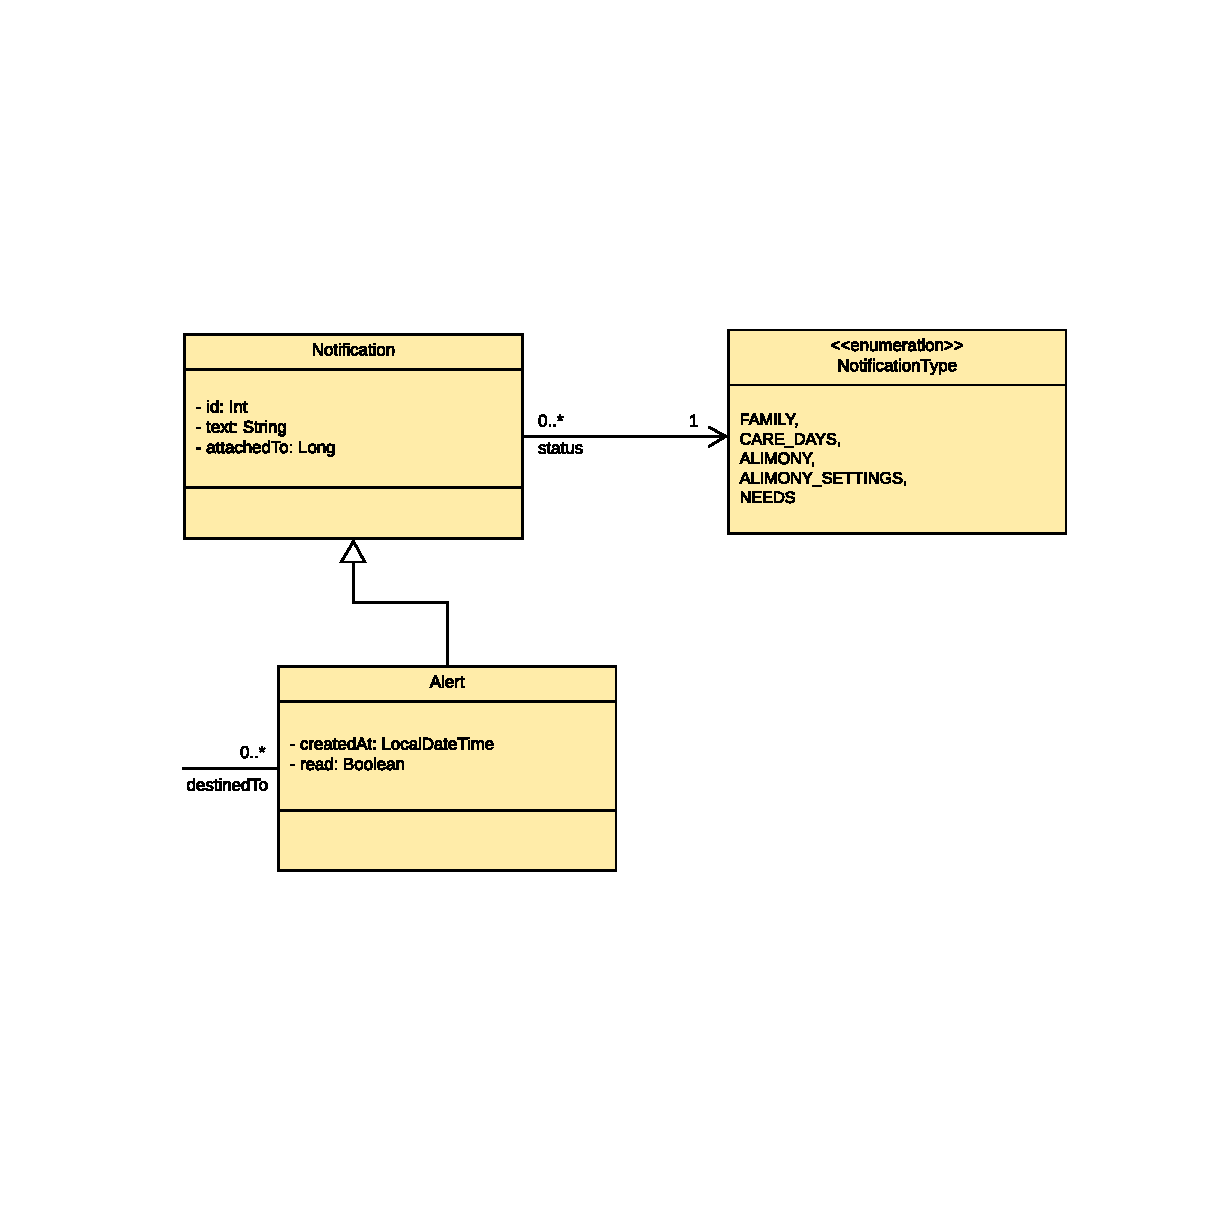
\includegraphics[width=1.0\textwidth]{pdfs/Notification2}
	       \caption[Nový návrh oznámení]{Nový návrh entity \texttt{Notification} a na ně se navazujících}\label{image:notification2}
        \end{figure}
        Předchozí návrh oznámení nebyl vhodný pro frontendovou část aplikace. Oznámení byla určena jenom pro konkrétní případ užití -- oznámení o~požadavku na změnu. Byla navržena obecně a neměla konkrétní typ. Tudíž oznámení elektronické pošty a upozornění v~telefonu byla reprezentována pomocí stejné entity.
        
        Předchozí abstraktní entita byla určena pro definování základních údajů. Zděděná entita definovala důležitost tohoto oznámení pro konkrétního uživatele a uživatele samotného. Bylo rozhodnuto zachránit abstraktní návrh entity \verb|Notification|, ale změnit jeho účel. Abstraktní entita bude obsahovat základní údaje pro všechny typy oznámení. Zděděné entity budou reprezentovat konkrétní typ oznámení.
        Současná implementace frontendové části aplikace vyžaduje zavedení typu upozornění, které by reprezentovaly upozornění v~rámci Android aplikace. Proto byla přidána entita \verb|Alert| (viz obrázek \ref{image:notification2}), která dědí základní údaje od entity \verb|Notification|. Pro zaručení konkretizace příčiny vytvoření oznámení byl přidán odkaz na událost, která je důvodem vzniku tohoto oznámení, do abstraktní entity a také typ této události. Typ oznámení je reprezentován pomocí entity výčtového typu -- \verb|AlertCause|. 
        Každá instance entity \verb|Alert| obsahuje atribut \verb|read| označující, jestli je oznámení přečteno uživatelem. Pro zaručení kvalitního návrhu API byla přidána možnost přečtení všech upozornění najednou. Přečtení upozornění je reprezentováno pomocí přidání atributu \verb|read| hodnoty \verb|true|.
        
        Výsledný návrh oznámení reprezentuje jednotlivá oznámení, která jsou dostupná pouze pro konkrétního uživatele. Přidané komentáře do oznámení jsou viditelné pouze pro adresáta příslušného oznámení, proto proces přidávaní komentářů byl odstraněn. Také byl přidán atribut \verb|text|, který je nutným pro~uvádění podrobnějšího popisu oznámení.
            
\section{Navržené změny}
    V~této sekci budou popsány změny navržené autorem této práce zaměřené na~vylepšení výsledné aplikace.
    
    \subsection{Interní DSL jazyk}\label{navrh:zmeny:dsl}
        % TODO popsat podrobneji
        \begin{figure}
            \begin{minted}[frame=lines,
        framesep=2mm,
        baselinestretch=1.2,
        fontsize=\footnotesize,
        linenos]{java}
/**
* Valid Interval with recurrence rule.
*/
private val validInterval = Interval(
        id = 1,
        interval_start = creationTime,
        interval_end = null,
        rRule = rule(frequency = Frequency.WEEKLY, count = 10) {
            byDays {
                and(DayOfWeek.MONDAY)
                and(DayOfWeek.WEDNESDAY)
                and(DayOfWeek.SUNDAY)
            }
        }
)
            \end{minted}
            \caption{Ukázka instance entity \texttt{Interval} s~pravidlem opakování} 
            \label{code:valid-interval}
        \end{figure}
        Pro pohodlné testování entit závislých na entitě \verb|Interval| byl implementován interní DSL\footnote{Domain Specific Language} jazyk, poskytující možnost vytvořit pravidlo opakovaní. Na obrázku \ref{code:valid-interval} je zobrazen příklad intervalu, který má pravidlo opakování vytvořené pomoci DSL jazyka. Příklad je převzat ze současné implementace testování.

    \subsection{Album}
        Libovolný člen rodiny může mít několik vlastních alb, která potřebuje rozlišovat mezi sebou. Předchozí návrh entity \verb|Album| neposkytoval možnost přidání názvu, proto do entity byl přidán příslušný atribut.
        
    \subsection{Konverter}
        V~sekci \ref{analyza:soucasnaImplementace} již bylo zmíněno, že pro implementaci serveru byla zvolena třívrstvá architektura. Doménová vrstva komunikuje s~datovou vrstvou pomocí tříd reprezentujících entity databáze, ale s~aplikační vrstvou tato komunikace probíhá pomocí DTO. Konverze mezi entitou a DTO se provádí v~této vrstvě. Za konverzi z~entity na DTO odpovídá třída entity. Za konverzi z~DTO na~entitu odpovídá třída DTO.
        Takový postup těsně provazuje entitu s~příslušnou třídou DTO, tennto problém se také nazývá \textit{tight coupling}. Zavedení konvertorů zmenšuje takovou závislost. Každý konvertor obsahuje metodu konvertující entitu na příslušné DTO a metodu konvertující DTO na příslušnou entitu. Takový postup umožňuje odstranit stejné metody z~příslušných tříd, což zvětšuje modularitu návrhu. 
        Pak je možné snadno přidat jiné DTO reprezentující stejnou entitu bez úprav entity samotné, a naopak.
        
        
        \begin{figure} % [H] TODO
            \begin{minted}[frame=lines,
        framesep=2mm,
        baselinestretch=1.2,
        fontsize=\footnotesize,
        linenos]{java}
internal interface InterfaceConverter<E : InterfaceEntity, D : InterfaceDTO> {

    fun convertToEntity(dto: D): E

    fun convertToDTO(entity: E): D

}
            \end{minted}
            \caption{Ukázka rozhraní \texttt{InterfaceConverter}} 
            \label{code:interface-converterl}
        \end{figure}
        Pro dosažení kvalitnějšího výsledku a zrychlení implementace bylo zavedeno rozhraní definující implicitní metody pro každý konvertor (viz obrázek \ref{code:interface-converterl}). Rozhraní také potřebuje zadání typu entity a DTO, které mají být podtřídami \verb|InterfaceEntity| a \verb|InterfaceDTO|. Tyto rozhraní nedefinují základní funkce, ale jenom označují typy těchto tříd. 
        
    \subsection{Našeptávač pro výjimky}
        Našeptávač pro výjimky byl zmíněn již v~sekci \ref{analyza:implementace:tridy}. Tato komponenta byla rozšířena o~typ výjimky označující, že DTO nebyl správně serializován kvůli nedostatku potřebných atributů. Příkladem může být překlep v~názvu povinného atributu. Také návratová zpráva byla rozšířena o~textový název chyby a časové razítko. Výslednou konfiguraci našeptávače najdete v~příloze \ref{dodatek:excpetion-handler2}.
        
    \subsection{Aplikační vrstva}
        V~předchozí implementaci byl použit POST požadavek, jak pro vytváření, tak pro aktualizaci. Tento požadavek očekává Data Transfer Object (DTO) v těle požadavku. Požadavky se rozlišují mezi sebou přítomností identifikátoru entity v DTO. Pokud je ID nastaveno na \verb|null| vytvoří se nový záznam v~databázi. V~opačném případě se server pokusí najít a aktualizovat záznam.
        
        
        Nový návrh aplikační vrstvy podporuje POST a PUT požadavky. POST požadavek je určen pro vytvoření nového záznamu a vyžaduje aby atribut \verb|id| v~DTO byl nastaven na hodnotu \verb|null|. PUT požadavek je určen pro aktualizaci záznamu a vyžaduje aby atribut \verb|id| v~DTO byl nastaven na číslo.
        
        
        Jeden uživatel může být současně členem několika různých rodin. Serverový backend nemůže předem vědět, ve které rodině se aktuálně uživatel nachází. Proto do API byly přidány požadavky, které vyžadují zadání identifikátoru konkrétní rodiny. Na základě tohoto identifikátoru se filtrují záznamy, které obdrží uživatel. Požadavky nevyžadující identifikátor rodiny nebyly odstraněny, protože všechny požadavky procházejí proces filtrace. Následně konečný uživatel obdrží jenom záznamy, které jsou pro něj dostupné.
        
        
        Dokumentace aplikační vrstvy byla též rozšířena o~návratové statusy pro každou metodu. Všechny parametry metod jsou získány z~požadavků, proto byly přidány i podrobné popisy parametrů metod. 
        
    \subsection{Doménová vrstva}%prejmenovat na ceskou verzi
        Nový návrh aplikační vrstvy rozděluje proces vytváření nových záznamů a proces aktualizace již existujících záznamů. Proto tento proces byl rozdělen do~dvou separátních procesů i v~doménové vrstvě.
        
        
        Proces filtrování záznamů podle aktuálně přihlášeného uživatele se provádí na datové vrstvě. Doménová vrstva jenom používá specifické metody datové vrstvy obsahující filtraci. V~případě, že požadovaná data nepatří konkrétnímu uživateli, ale celé rodině, provádí se ověření, jestli aktuálně přihlášený uživatel patří do této rodiny.
        
    \subsection{Datová vrstva}
        V~předchozí implementaci datové vrstvy byly použity implicitní metody, které poskytuje framework Spring Data. V~současné implementaci byly přidány vlastní metody s~použitím nástroje pro vytváření metod dotazování (\textit{query methods}). Přidané metody jsou zavedeny za účelem filtrování záznamů, které obdrží uživatel. Filtrování se provádí na základě údajů o~aktuálně přihlášeném uživateli.
        V~případě, že požadované záznamy nepatří konkrétnímu uživateli, ale celé rodině, ověřuje se, jestli aktuálně přihlášený uživatel patří do této rodiny.
    
    \subsection{Implementace historie změn}
        Důležitou částí aplikace je zaznamenání změn udělaných uživatelem. Úpravou je změna záznamu entity, kterou uživatel s~rolí \enquote{ROLE\_USER} může upravit. Takovou roli má jakýkoliv uživatel přihlášený do systému. Aktivita \texttt{root}\footnote{Uživatel s~rolí \enquote{ROLE\_ROOT}.} uživatele není uvažována, protože tento uživatel není přítomný v~rámci profilu pro produkci. Příkladem takové změny může být změna nastavení alimentů nebo označení oznámení jako přečtené.
    
        Historie změn ještě nebyly implementovány, ale návrh již existoval a hlavní myšlenka zůstává stejná. Záznam historie kopíruje všechny atributy entity a přidává čas vytvoření záznamu a vlastní identifikátor\footnote{Identifikátor v~rámci databáze.}. Entita \verb|History| je abstraktní třídou, neboli generalizací v~případě návrhu v~doménovém modelu. Jednotlivé entity, které jsou zděděné od této entity, reprezentují historie příslušných entit (viz obrázek \ref{image:History1}). 
    
        Tato entita byla implementována jako poslední a všechny změny, které se jí týkají, jsou srozumitelné jenom po přečtení všech změn návrhu. Nejprve bylo potřeba upravit návrh podle implementovaných změn v~příslušných entitách a až poté začít s~návrhem vhodných změn této entity (viz obrázek \ref{image:History1_2}).
        
        Dalším krokem úprav je navržení úprav, které už nejsou nutné, ale výrazně zlepšují výsledný návrh programu:
        \begin{itemize}
            % \setlength\itemsep{0.3em}
            \item přidání do každé entity reprezentující historii odkazy na příslušné entity, například entita \texttt{AlimonyHistory} bude mít navíc odkaz na entitu \texttt{Alimony};
            \item zavedení nové entity historie \texttt{CareDaysSettingHistory} podle návrhu entity \texttt{CareDaysSetting}, která byla popsána v~sekci \ref{navrh:upravy:caredays}.
        \end{itemize}
        %TODO image
        Výsledný návrh entity \verb|History| (viz přílohu \ref{dodatek:DomainModel2}) byl kompletně implementován. Také byly přidány řadiče pro každý typ historie, které poskytují možnost vyhledat záznamy. Uživatel nemůže vytvořit nový záznam historie nebo změnit již existující záznam. Proto API serveru nepodporuje příslušné požadavky. Vytvoření instancí historie se provádí serverem automaticky při aktualizacích příslušných entit.
        Spravování entit historie v~doménové vrstvě bylo rozděleno do dvou logických bloků. První blok se zabývá spravováním požadavků Android aplikace. Každý typ historie má vlastní rozhraní reprezentující metody, které je možné provádět s~touto entitou. Druhým logickým blokem je proces vytváření instancí historie. Za tímto účelem bylo přidáno rozhraní \verb|InternalHistoryService|, které poskytuje metodu \verb|toHistory| pro uložení instance do databáze.
        Metoda očekává jako parametr instanci třídy před provedením změn a konvertuje tuto instanci do příslušné instance historie. Každý typ historie má též vlastní konvertor z~entity do entity historie. Například, po~vložení do metody \verb|toHistory| parametru typu \verb|Bill|, bude zavolán konvertor \verb|BillToHistoryConvertor|, který vrátí instanci třídy \verb|BillHistory|. 

\section{Návrh bezpečnosti}\label{navrh:bezpecnost}
    \subsection{OAuth 2.0}
        % TODO
        Za účelem zabezpečení procesu autorizace byl zvolen protokol OAuth 2.0. Tento protokol je nativně podporován frameworkem Spring. Proto byla provedena jeho konfigurace, která vyžadovala implementaci následujících rozhraní:
        \begin{itemize}
            % \setlength\itemsep{0.3em}
            \item \texttt{UserDetailsService} -- pro definování zdroje informací o~uživatelích;
            \item \texttt{WebSecurityConfigurerAdapter} -- pro definování implementace rozhraní \texttt{UserDetailsService} a nastavení kontextu bezpečnosti;
            \item \texttt{AuthorizationServerConfigurerAdapter} -- pro nastavení procesu přihlašování;
            \item \texttt{ResourceServerConfigurerAdapter} -- pro nastavení přístupu do řadičů.
        \end{itemize}
        
        Rozhraní \verb|UserDetails| bylo implementováno pro každý profil zvlášť. Pro pohodlný proces vývoje byl přidán uživatel s~rolí \enquote{ROLE\_ROOT} pro profil \verb|dev|. Za účelem testování byly přidány implicitní uživatele pro profil \verb|test|. Třetí implementace byla provedena pro profil produkce, proto žádného implicitního uživatele tato implementace nemá.
        
    \subsection{HTTPS}
        V~předchozí implementaci aplikace byl použit protokol HTTP\footnote{Hypertext Transfer Protocol}, který nezaručuje bezpečnou komunikaci mezi klientem a serverem. Proto tento protokol byl nahrazen protokolem HTTPS\footnote{Hypertext Transfer Protocol Secure}, který vyžaduj certifikát podepsaný třetí stranou. Tento certifikát je uložen v~aplikaci.
        
\section{Profily}\label{navrh:profily}
    Během implementace serveru byla potřeba rozšířit návrh profilů aplikace. Původní návrh obsahoval jenom implicitní profil a profil vývoje, obsahující konfiguraci databáze H2. Výsledný návrh aplikace potřebuje více profilů, proto byly přidány dva další profily: profil pro produkci a profil pro testování. Důvodem přidání dalších profilů jsou rozdíly mezi konfiguracemi, které potřebují konkrétní případy spouštění aplikace. Princip chování profilu byl již zmíněn v~sekci \ref{analyza:soucasnaImplementace:profily}, proto v~této sekci budou popsané provedené změny.
    
    Pro podrobnější popis přidaných profilů je potřeba nejdřív popsat výslednou konfiguraci existujícího profilu vytvořeného pro proces vývoje. Seznam provedených změn a rozšíření, které navazují na tento profil:
    \begin{itemize}
            % \setlength\itemsep{0.3em}
            \item Rozšířena konfigurace databáze. Změny byly provedeny za účelem přesnější definice konfigurace (viz sekci \ref{navrh:db});
            \item Přidána nutná konfigurace pro bezpečnost aplikace, která byla popsána v~sekci \ref{navrh:bezpecnost};
            \item Přidána proměnná do konfiguračního souboru, která zapíná pravidelné vytváření alimentů (viz sekci \ref{navrh:upravy:alimenty}) a také proměnná definující pravidlo, podle kterého se řídí plánování spouštění této třídy;
            \item Přidána specifická implementace pro rozhraní \textit{UserDetails} (viz sekci \ref{navrh:bezpecnost});
            \item Přejmenován profil \enquote{development} na \enquote{dev}, za účelem lepší přehlednosti kódu při definování několika profilů komponenty najednou.
    \end{itemize}
    
    Výše uvedená konfigurace je vhodná pro vývoj aplikace, ale zároveň není vhodná pro produkci a testování aplikace. Proto bylo rozhodnuto nechat v~implicitním konfiguračním souboru jenom definici profilu, který by měla aplikace využít pro následující spuštění, a přidat další profily podle případů užití.
    
    Prvním profilem, který byl přidán, je profil pro produkci. Hlavním rozdílem tohoto profilu od profilu vývoje je použitá databáze. Podrobněji bude zvolená databáze popsána v~sekci \ref{navrh:db}. Pro tuto sekci je postačující zmínit, že zvolená databáze je PostrgeSQl. Druhou odlišností je jiná implementace rozhraní \verb|UserDetails|. Produkční verze aplikace by neměla mít \verb|root| uživatele. Jiný konfigurační soubor také dovoluje nechat konfiguraci pro produkci nedotčenou při možném velkém počtu změn v~jiných profilech.
    Například, můžeme nechat vypnuté plánované vytváření alimentů pro vývojový profil.
    
    Druhým profilem, který byl přidán do aplikace, je profil pro testování. Změny se dotkly stejných aspektů jako profilu produkce. Byla přidána nová implementace rozhraní \verb|UserDetails|, která obsahuje implicitních uživatele s~různými rolemi. Také byla přidána konfigurace databáze. Pro tento profil byla zvolena stejná databáze jako i pro profil produkce. Takový postup zmenšuje šance na~výskyt nečekaných chyb, působených použitím odlišné databáze v~produkci.
    
\section{Databáze} \label{navrh:db}
    Použité databáze byly popsány v~sekci \ref{resere:databaze}. V~této sekci bude vysvětleno, proč byly zvoleny tyto databáze.
    
    Profil pro vývoj používá databázi H2. Stejná databáze byla použita při předchozí implementaci. Databáze nevyžadovala její nahrazení jinou databází, protože nevyžaduje nastartování databáze zvlášť od aplikace, ale nastartuje se~spolu s~aplikací. Všechna data se ukládají přímo v~paměti aplikace, proto po~restartování aplikace smaže všechny vytvořené záznamy.
    
    Pro profil produkce bylo rozhodnuto použít jinou databázi. Volilo se mezi dvěma databázemi: PostgreSQL a MySQL. Tyto databáze jsou jedny z~nejpopulárnějších databází v~současné době a zároveň jsou otevřeným softwarem. Po~porovnání těchto dvou databází, byla vybrána databáze PostgreSQL. Některé funkce byly považovány za důležité přesto, že ještě nebyly využity v~implementaci a návrhu. Příklady převah PostgreSQL nad MySQL: 
    \begin{itemize}
            % \setlength\itemsep{0.3em}
            \item PostgreSQL je objektově relační databáze \cite{postgres-about}, zato MySQL je pouze relační databáze. To znamená, že PostgreSQL dovoluje dědění tabulek a přetěžování metod;
            \item PostgreSQL poskytuje možnost definovat vlastní typy \cite{pstgres-create-type};
            \item autor této práce má zkušenosti s~PostgreSQL.
    \end{itemize}
    Informace o~rozdílech těchto databází byly převzaty z~několika článků na internetu. Nejpoužitelnějšími pro autora této práce byly \cite{mysql-postgres1, mysql-postgres2}.
    
    
\section{Návrh testování}\label{navrh:testovani}
    Pro testování kódu budou využity frameworky JUnit 5 a Spring. Tyto frameworky byly podrobně popsány v~sekci \ref{reserse:testovani}. Testování se skládá s~\texttt{unit}\footnote{Testy, zaměřené na ověření správnosti fungování samostatně testovatelných částí programu.} testů a \texttt{integračních}\footnote{Testy, zaměřené na ověření správné komunikace mezi komponentami.} testů. Návrhy testů se budou podstatně lišit mezi sebou. Proto budou využité funkce poskytované frameworkem JUnit 5, který od verze 5 poskytuje možnost označovat testy pomocí tagů.\cite{junit-tags} Podrobnější informace o~implementaci tagů budou uvedeny v~sekci \ref{testovani:tagy}. Kompletní implementace testování bude popsána v~kapitole \ref{chapter:testovani}.
    
    \subsection{Unit testy}
        Unit testy využívají pouze funkce frameworku JUnit 5 a testují základní funkce. Otestovány mají byt třídy a metody, které mohou být otestovány samostatně. Tyto testy také mají být označeny jako unit testy pomocí tagů.
        
    \subsection{Integráční testy}
        Integrační testy budou testovat jednotlivé řadiče. Tyto testy jsou navrženy pomocí principu IoC a budou označeny jako integrační testy a zároveň jako pomalé testy.

\section{Implementace bezpečnosti}
        V~současné implementaci je autorizační server součástí serverového backendu a odpovídá jak za registraci uživatele, tak i za přihlášení. Pro registraci má uživatel poslat DTO se svými údaje na příslušný řadič\footnote{Řadič je namapován na cestu \enquote{/api/v1/aut}.}. Pro přístup do zmíněného řadiče se používá typ přístupu \textit{user credentials}. Uživatel potřebuje uvést adresu pro obdržení \textit{tokenu}\footnote{Alfanumerické heslo.}, identifikátor uživatele a \textit{secret}. Potom uživatel obdrží \textit{tokeny} umožňující provést registraci.
        Pro přihlašování uživatele se používá typ obdržení průkazů \textit{resource owner password credetials}, kde uživatel potřebuje, navíc od předchozího typu, poslat svoje uživatelské jméno a heslo. Potom uživatel obdrží \textit{access token}\footnote{Tento \textit{token} klient používá pro komunikaci se serverem.} a \textit{refresh token}\footnote{Tento \textit{token} klient používá pro obnovení \textit{access tokenu} po vypršení jeho platnosti.} jako návratové hodnoty. Platnost \textit{tokenu} pro komunikaci je omezen jednou hodinou. Platnost \textit{tokenu} pro obnovení \textit{access tokenu} pro komunikaci je omezen jedním týdnem.